\begin{tikzpicture}
%\draw[step=0.5, gray, very thin] (0,0) grid (10, 7);

\def \sRight {0}

\node[inner sep=0pt] (russell) at (5 +\sRight, 5)
    {\includegraphics[width=.30\textwidth]{LSTM.png}};

\node[inner sep=0pt] (russell) at (5 +\sRight, 2)
    {\includegraphics[width=.33\textwidth]{GRU.png}};

\node[inner sep=0pt] (russell) at (9.7 +\sRight, 4)
    {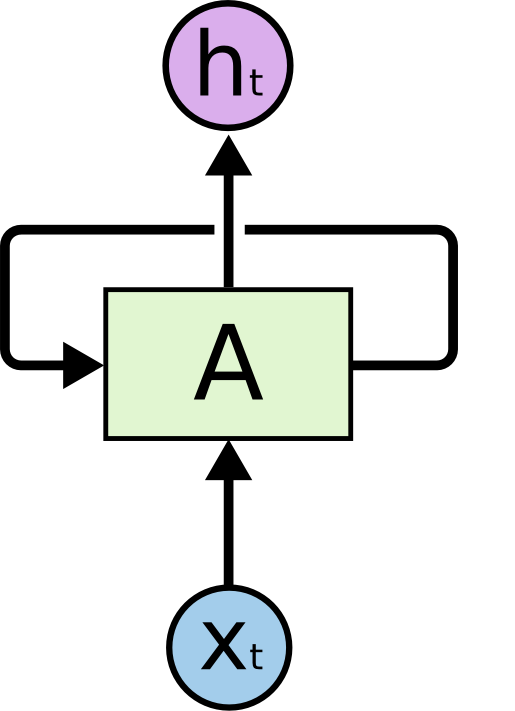
\includegraphics[width=.30\textwidth]{rolledRNN.png}};

\draw[arrows=-angle 90, line width=2pt, myBlue2]  (8.5, 3.7) -- (6.5, 4.75);
\draw[arrows=-angle 90, line width=2pt, myBlue2]  (8.5, 3.5) -- (6.5, 1.75);


\node at (3, 4.4) {\tiny  $h_{t - 1}$};
\node at (3, 5.4) {\tiny  $C_{t - 1}$};

\node at (6.8, 4.4) {\tiny  $h_{t}$};
\node at (6.8, 5.4) {\tiny  $C_{t}$};
%\node[draw,text width=9cm] at (0, 6) {
%   \begin{minipage}{9cm}
%    \small
%        \begin{align*}
%          f_t  &= \sigma(W_f  x_t + U_f h_{t-1} + b_t)\\
%          i_t  &= \sigma(W_i  x_t + U_i h_{t-1} + b_i)\\
%          o_t  &= \sigma(W_o  x_t + U_o h_{t-1} + b_o)\\
%          C_t  &= f_t \circ c_{t-1} + i_t \circ tanh(W_c x_t + U_c h_{t-1} + b_c)\\
%          h_t  &= o_t \circ tanh(c_t)
%        \end{align*}
%    \end{minipage}
%};


\node at (2.3, 5) {LSTM unit};
\node at (2.3, 1.8) {GRU unit};
\end{tikzpicture}

